\section{Dynamic updates}
\label{dynamic}

This section describes update procedures of both \inducedgraph{} and \treeindex{} in dynamic graphs. We focus on edge insertion/deletion as vertex insert/deletion can be represented by inserting/deleting an isolated vertex and several following edge insertions/deletions.

The scope of affected edges when a new edge is inserted/deleted has been well studied in~\cite{huang2014querying}. When an edge $e_0$ has been added/removed from $G_o$, the affected edges, \ie with trussness changes, are either directly forming new triangles of weight $\ge \tau_{e_0}$ or are triangle connected to the new edge $e_0$ with all triangles of weight $\ge \tau_{e_0}$. With this rule, the authors of~\cite{huang2014querying} also developed an efficient algorithm to calculate edge trussness updates. 

We can then proceed to update the \inducedgraph{} $G_m$ once edge trussness in $G_o$ have been updated. For the insertion of an edge $e_0$, a new vertex $x_0$ is added to $G_{m}^{prime}$ with several new adjacent edges and updated weight of some vertices and edges. All we need to do is maintain the maximum spanning tree $G_m$ with these changes in $G_{m}^{prime}$. As maintaining Minimum spanning tree is a well studied area with highly efficient algorithms~\cite{cattaneo2002maintaining}, we omit the details here.

\note{are there problems if we dont update vertex and edges in order?}
Once we have updated $G_m$, we can proceed to update the \treeindex{} $G_t$. There are two types of changes for the update of $G_m$. One is vertex based that includes adding the new vertex $x_0$ and updating weights of other affected vertices. For a vertex $x$ that have updated weight, according to \autoref{thm:\inducedgraph{}_vertex_trussness}, the algorithm needs to create a new child vertex of current vertex $h[x]$ in $G_t$ based on the new weight. Note that this update is incomplete in the sense that we haven't taken into account the weight changes of the adjacent edges.  

\begin{algorithm}
	\KwData{An inserted/updated edge $(x, y) \in G_{m}$}
	\KwResult{None}
	\BlankLine
	$C_x \gets h[x]$, $C_y \gets h[y]$\;
	$k \gets w_{(x,y)}$\;
	\lWhile{$\tau_{C_x} > k$} {
		$C_x \gets C_{x}.parent$
	}
	\lWhile{$\tau_{C_y} > k$} {
		$C_y \gets C_{y}.parent$
	}
	$C \gets \emptyset$ \Comment{Assume $\tau_{\emptyset} = -1$.}\;
	\While{$C_x \neq \emptyset$ \textbf{or} $C_y \neq \emptyset$}{
		\uIf{$\tau_{C_x} > \tau_{C_y}$} {
			\lIf{$C \neq \emptyset$} {$C.parent \gets C_x$}
			$C \gets C_x$, $C_x \gets C_{x}.parent$\;
		}
		\uElseIf{$\tau_{C_x} < \tau_{C_y}$} {
			\lIf{$C \neq \emptyset$} {$C.parent \gets C_y$}
			$C \gets C_y$, $C_y \gets C_{y}.parent$\;
		}
		\Else{
			$C_c \gets$ combine ($C_x$, $C_y$)\;
			\lIf{$C \neq \emptyset$} {$C.parent \gets C_c$}
			$C \gets C_c$, $C_x \gets C_{x}.parent$, $C_y \gets C_{y}.parent$\;
		}
	}
	\caption{Zipper (Combine two branches)}\label{alg:zipper}
\end{algorithm}

Another type of change is that a new edge is added to $G_m$ or an edge has updated weight. This happens when a new triangle is formed in $G_o$ or the lowest trussness of edges in a triangle has changed. For a new edge $(x,y)$ in $G_m$, if $x$ and $y$ belongs to different connected components in $G_m$, then we need to combine the two branches of trees to which $h[x]$ and $h[y]$ belongs. We call this procedure zipper as shown in \autoref{alg:zipper}. In this way, K-Truss communities with trussness lower than the weight of the edge are combined together and the rest of high trussness communities become two separate children branch. An example is shown in \autoref{fig:dynamic_update}.

\begin{figure}[ht]
    \centering
    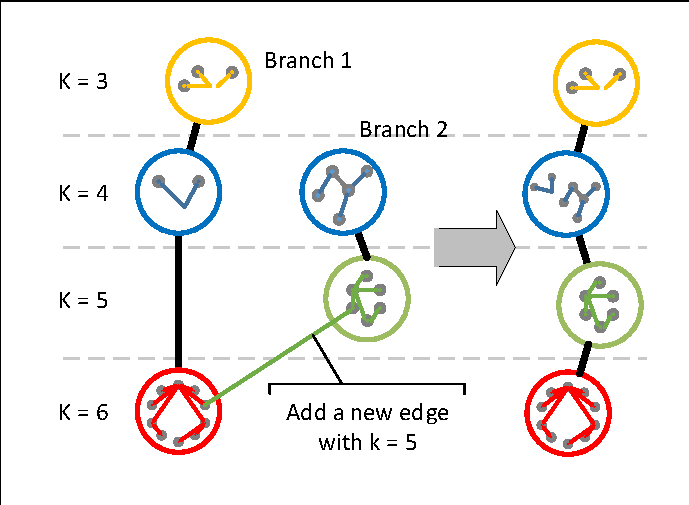
\includegraphics[width=\linewidth]{./figures/dynamic_update.pdf}
    \caption{An example or zipper operation when adding a new edge.}
    \label{fig:dynamic_update}
\end{figure}

\note{add a theorem here?} 
However, if a new edge is inserted in $G_m$ without join two disconnected parts, another edge with lower weight in $G_m$ must have been deleted to maintain the minimum spanning tree. In this case, if the two ends of the new edge $h[x]$ and $h[y]$ is different, we can still use zipper procedure to combine these two branches. The only difference is that we need to apply the zipper procedure from the least common ancestor of $h[x]$ and $h[y]$. Same goes for an edge with updated weight, as it can be viewed as deleting the edge with old weight and inserting a new edge with updated weight.

The update procedure for edge deletion in $G_o$ follows a similar process. It involves a vertex removal and vertex weight decreasing as well as several edge deletion and edge weight decreasing in $G_m$. Similarly, in $G_t$, we use a procedure to 'unzip' the branch of a deleted edge into two separate branches or a partially separated branch.

When using the zipper procedure to combine two branches (or divide one branch), we may have performance issues when updating the hashtable $h$. As one vertex change in $G_t$ may involve several entries to be updated in $h$. So how do we solve this problem....

\note{add time complexity analysis}

%Based on the update of the \inducedgraph{} $G_m$, we can update the \treeindex{} $G_t$. 
%\begin{itemize}
	%\item \textbf{Add a new edge in $G_o$} Add a new vertex in $G_m$. So only need to add a new vertex and create its own k-truss community in $G_t$ as it is not connected to any component in $G_m$ now.
	%\item \textbf{Form a new triangle in $G_o$} Add a new edge in $G_{m}^{prime}$. If such an edge is updated into the MST $G_m$, there might be another edge that has been deleted from $G_m$. However, in such a case, the connected components are still the same. But no matter the new edge connect two formerly disconnected components or not, the algorithm runs the same way. The algorithm can now combine two branch of the tree (or tree in case it connects two disconnected components) together. How? \note{define a procedure here} First find the LCA, and then check from the LCA, add each node with the lowest k from both side. If there are two nodes that has same k, combine them and add the combined node to the tree.
	%\item \textbf{a triangle has trussness update in $G_o$} An edge has weight update in $G_{m}^{prime}$. If such an edge does not belongs to $G_m$ previously, and now becomes an edge in $G_m$, same as adding a new edge. Otherwise, As from \autoref{thm:\inducedgraph{}_vertex_trussness}
	%
%\end{itemize}
